\chapter{Grundlagen}
\label{cha:Grundlagen}


\section{Benchmarking}

Das Vergleichen der Performanz verschiedener Systeme anhand von Messungen wird als \textit{Benchmarking} bezeichnet. 
Die in diesen Messungen verwendeten Workloads sind standardisiert und werden \textit{Benchmarks} genannt \cite{defi_benchmarking}.
Mit Systeme ist hier gemeint, dass es die Hardware wie CPU/GPU \cite{wang2019benchmarkingtpugpucpu} oder Harddrives \cite{ssd_benchmark} getestet werden oder auch Software 
wie VMs \cite{statistically_rigorous}. Um solche Benchmarks durchzuführen werden Benchmarkingtools verwendet, um Messungen und am Ende Vergleiche stellen zu können.
Das Tool was in dieser Arbeit verwendet ist das Fio-Tool.

\subsection{Fio-Tool}
Das fio\footnote{flexible Input Output} \cite{axboe} Benchmarking-Tool arbeitet in der Konsole und es gibt kein UI.
Um das Programm auszuführen werden zusätzlich Parameter verwendet.
Um einen Festplattenbenchmark-Test selber durchzuführen, sieht der Command wie folgt aus:

\begin{lstlisting}[caption=Beispiel für eine Ausführung eines fio-jobs, label={lst:job}]
  ./fio --rw=write --runtime=2s --write_bw_log=mytest --name=test --size=1024m
\end{lstlisting}


\begin{center}
  \begin{table}[h!]
    \begin{tabularx}{\textwidth}{|X|X|}
      \hline
        \textbf{Parameter}& \textbf{Definition} \\ 
      \hline
      fio & Das fio Executable  \\ 
      \hline
      rw=write & Auswahl von read oder write des Tests  \\ 
      \hline
      runtime=2s & Maximale Dauer eines Tests  \\ 
      \hline
      write\_bw\_log=mytest &  Name des Logs die ausgeben werden soll   \\ 
      \hline
      name=test &  Name des Tests   \\ 
      \hline
      size=1024m & Größe der Datei für den read/write Test    \\ 
      \hline
    \end{tabularx}
    \caption{Beispiel Command zur Ausführung des Fio-Tools}
    \label{tab:1d_1_sta}
  \end{table}
\end{center}

Solche Command kann auch in eine Datei geschrieben, was die .fio Datei sind. In dieser Arbeit wird so eine Ausführung als einen \textit{Job} bezeichnet.
Der Job oben testet das Random Read mit einer Laufzeit (Runtime) von 2 Sekunden und liest eine Datei mit einer Größe von 128 Mebibyte. Dieser Job wird nur einmal durchlaufen. 
Für einen wiederholten Lauf gibt es den Parameter loop, wo zusätzlich die Anzahl angegeben wird, wie oft dieser \textit{run} wiederholt werden soll.
So ist ein Job ein abgeschlossener Durchlauf von allen \textit{runs}.
Wenn der Job abgeschlossen ist und der Parameter write\_bw\_log verwendet wurde, gibt das fio-Tool ein log Datei von dem ausgeführten Job.

\begin{lstlisting}[caption=Erste Zeilen des Logs (Bezeichnungen sind nicht im Log enthalten),label={lst:log_line_example}]
  [Time,	Bandwidth,    data direction, Blocksize,	Offset]
  0, 	    59782,        0,		            4096,		    0
  0, 	    54353,        0,		            4096,		    0
  1, 	    45545,        0,		            4096,		    0
\end{lstlisting}

Time für die Zeit in Millisekunden (ms) die verlaufen ist, Bandwidth für die
Bandbreitengeschwindigkeit in Kibibyte/s, der dritte Wert für die data direction,
 ob gelesen (= 0) oder geschrieben (= 1) wurde und ein Blocksize und
ein Offset. Die Logdaten selbst könne über 10.000 Zeilen umfassen und sind
daher schwer lesbar

\subsection{Warmup und stationärer Zustand}
Der stationärer Zustand ist ein Muster, das sich mit der Zeit wiederholt und bei dem das Verhalten in einem Zeitraum von der 
gleichen Natur ist wie in jedem anderen Zeitraum \cite{transient_state_definition}. Um zu ermitteln,
wann der stationäre Zustand eingetreten ist, sind stabile Messwerte erforderlich.

Bevor aber der stationäre Zustand erfolgt, ist ein Warmup erforderlich.
Dieser Warmup wird auch als transiente Zustand bezeichnet.
Ein transientes Verhalten beschreibt jene Veränderungen, bei denen sich der Charakter des Systems im Laufe der Zeit verändert \cite{transient_state_definition}.

Bei Hardware oder Software ist anfangs wiederholtes testen notwendig, um
sie analysieren zu können. 
Ein Beispiel wo die Hardware einen Warmup braucht sind die Caches beim Festplattenbenchmarking \cite{nine-year-of-bench}
% Seite 6 "warm" "cold" caches
Erst nach diesen Warm-ups wird der
stationäre Zustand der Performanz (engl. steady state of peak performance)
erreicht.

Hindernisse bei den Messungen in Benchmarking sind nicht-deterministische Faktoren.
Als Beispiel, ein wiederholtes Lesen/Schreiben auf demselben System mit derselben Datei, erreicht im Durchschnitt nicht ein konstante Bandbreitengeschwindigkeit. 
Sie wird immer abweichen. Ursachen dafür könnten schon verschiedene CPU-Temperaturen sein, 
aber auch CPU-Scaling oder parallele Prozessierung [7]. Das Fio
selbst arbeitet nicht nur mit einem Thread, sondern es arbeitet mit Multi-
threads, was nicht-deterministische Zustände hervorrufen kann. Weitere nicht-
deterministische Faktoren sind die Caches die beim Lesen oder Schreiben ver-
wendet werden, je nach dem ob sie leer sind oder schon beschrieben wurden.
Auch nicht essentielle Prozesse (oder auch essentielle Prozesse wie Daemons3),
die immer Hintergrund laufen, können die Geschwindigkeit beeinflussen [15].
Da der Nichtdeterminismus Schwankungen in den Messungen verursacht, müssen dies in Betracht gezogen werden.

Da sich die Geschwindigkeit nie konstant einem Wert nähert, sondern stets
abweicht, soll das Analysetool in Zukunft mit statistischen Tests mit der zusätzlichen Fehlerrate den stationären
Zustand ermitteln und dabei den Nichtdeterminismus berücksichtigen.

Doch die Auswahl der Runs aus den Tests für die Bestimmung des stationäre Zustand trägt zu einer signifikante Entscheidung bei,
 ob der transiente Zustand abgeschlossen ist.
Die Auswahl der Logs und deren Diese Auswertung können signifikante Unterschiede aufweisen, die die Evaluierung
verändern würden \cite{when_stop_tests}.



\section{Statistische Analyse/Tests}
Es werden verschiedene Tests verwendet um herauszufinden ob eine Performanzänderung vorliegt \cite{statistically_rigorous}
Die Grundgesamtheit wird ein fio-Job sein und die Stichproben werden die Iteration/Runs sein die für die Tests entnommen werden.
Diese statistische Tests werden genutzt, um zu ermitteln ob eine statistische Signifikanz zwischen den Stichproben vorhanden ist.

Wenn die statistisch Signifikanz erfüllt ist, wird die Nullhypothese abgelehnt \cite{inferenzstatistik}.
Die Nullhypothese ist hier die Annahme, dass es zwischen den Logs keine Abhängigkeit besteht und zufällig entstanden sind.
Somit ist die Alternativhypothese, dass zwischen den ausgewählten Stichproben ein Zusammenhang/Abhängigkeit besteht.
Die verwendeten Tests wie der t-Test und Tests mit Konfidenzintervallen haben die Bedingung, 
dass die Stichprobe einer Normalverteilung\footnote{auch Gaußverteilung} unterliegen \cite{inferenzstatistik}. 

Das Ablehnen der Nullhypothese, obwohl die Hypothese erfüllt ist, wird als Typ-1-Fehler bezeichnet.
Die Wahrscheinlichkeit dafür wird als $\alpha$ und als Signifikanzniveau bezeichnet. 
Zusätzlich mit den p-Werten (Signifikanzwahrscheinlichkeit) aus den statistischen Tests, wird die Statistische Signifikanz überprüft.
Dabei ist Der Wert p ist also nichts anderes als die (bedingte) Wahrscheinlichkeit der erhobenen oder
noch extremerer Daten, wenn die H0 als gültig angenommen wird \cite{inferenzstatistik}

\section{Normalverteilung/Gaußverteilung}

Die hier verwendet Tests, wie der T-Test und das quantifizieren eines Konfidenzintervalls, 
haben die Bedingung, dass sie einer Normalverteilung unterliegen müssen \cite{inferenzstatistik}.
Die Normalverteilung ist ein Dichtefunktion die einer Glockenform entspricht.
Die Funktion wird aus zwei Parametern zusammen. Die Varianz $\sigma^2$ und der Erwartungswert $\mu$.
Ist eine Zufallsvariable $X$ normalverteilt, kann sie mit der folgenden Formel beschrieben werden:

\begin{center}
  $X \sim N(\mu,\sigma^2)$
\end{center}

Dabei bedeutet hier "$\sim$" das Symbol, dass die Zufallsvariable $X$ normalverteilt ist.
Die Funktion $N$ verwendet die eigentliche Dichtefunktion:

\begin{center}
  $f(x) = \dfrac{1}{\sqrt{2\pi\sigma^2}} \cdot e^{-\frac{(x-\mu)^2}{2\sigma^2}}$
\end{center}

Die ausgewählten Stichproben werden die Runs aus einem fio-Job sein.
Damit spätere Tests auch durchgeführt werden können, wird der Zentralegrenzwertsatz genutzt, um diese Bediungen der Normalverteilung zu erfüllen.
Die Stichproben $n > 30$ Messwerte besitzen, somit ist der Zentrale Grenzwert erfüllt, denn dieser Satz sagt aus, 
Setzt sich eine Zufallsvariable additiv aus einer großen Zahl beliebig verteilter, stochastisch unabhängiger
Zufallsvariablen zusammen, so ist sie selbst näherungsweise normalverteilt \cite{statistically_rigorous}.
Eine spezielle Form für die Normalverteilung ist die Standardnormalverteilung.
Für diese Verteilung gilt das der Erwartungswert $\mu = 0$ und die Standardabweichung $\sigma^2 = 1$ ist.


\section{Varianzanalyse - Analysis of Variance (ANOVA)}
 
Dieses Kapitel führt eine allgemeine statistische Analysetechnik ein, die als Varianzanalyse (ANOVA) bezeichnet wird \cite{Lilja_2000}. 
ANOVA unterteilt die gesamte beobachtete Variation in einer Reihe von Messungen in mehrere Komponenten.
Diese Komponenten sind SSA\footnote{SSA - Sum of Squared errors of All treatment} (auch SSB \footnote{SSB - Sum of squares between}) und SSE\footnote{SSE - Sum of Squared Errors of all observation}
 (auch SSW\footnote{SSW - Sum of squares within}).
Die SSA  ist die quadratische Abweichung der Mittelwerte vom Gesamtmittelwert und die SSE
ist die gesamte Abweichung von den Mittelwerten in den Gruppen.
Das Ziel der Komponenten ist, festzustellen, ob die beobachteten Unterschiede zwischen den Mittelwerten der einzelnen Alternativen auf tatsächliche 
Unterschiede zwischen den Alternativen zurückzuführen sind oder ob sie lediglich Messfehler sind.
Die Alternativen hier werden die Iterationen eines fio-jobs sein.
Die Varianzanalyse geht davon aus, dass die Fehler in den Messungen für die verschiedenen Alternativen
unabhängig voneinander und normalverteilt sind, was mit dem Zentralen Grenzwertsatz erfüllt ist.
Die Messwerte für das Analysetool sind I/O-Geschwindigkeiten.
Es geht weiter davon aus, dass die Varianz der Messfehler bei allen Alternativen gleicher Art sind.
Die Tabelle \ref{tab:measurements} zeigt die Vorbereitung einer Varianzanalyse für einen fio-job.

\begin{table}[h!]
  \centering
  %\resizebox{\textwidth}{!}{
  \begin{tabular}{|c|*{5}{c}|c|}
  \hline
  \textbf{Messwerte} & \multicolumn{5}{c|}{\textbf{Iterationen/Alternativen}} & \textbf{Gesamtmittelwert} \\
  \cline{2-6}
   & 1 & 2 & $\cdots$ & $j$ & $k$ & \\
  \hline
  1 & $y_{11}$ & $y_{12}$ & $\cdots$ & $y_{1j}$ & $y_{1k}$ & \\
  2 & $y_{21}$ & $y_{22}$ & $\cdots$ & $y_{2j}$ & $y_{2k}$ & \\
  $\vdots$ & $\vdots$ & $\vdots$ & $\ddots$ & $\vdots$ & $\vdots$ & \\
  $i$ & $y_{i1}$ & $y_{i2}$ & $\cdots$ & $y_{ij}$ & $y_{ik}$ & \\
  $\vdots$ & $\vdots$ & $\vdots$ & $\ddots$ & $\vdots$ & $\vdots$ & \\
  $n$ & $y_{n1}$ & $y_{n2}$ & $\cdots$ & $y_{nj}$ & $y_{nk}$ &  \\
  \hline
  Spaltenmittelwert & $\bar{y}_{\cdot1}$ & $\bar{y}_{\cdot2}$ & $\cdots$ & $\bar{y}_{\cdot j}$ & $\bar{y}_{\cdot k}$ & $\bar{y}_{\cdot \cdot}$ \\
  %Effekte & $\alpha_{\cdot 1}$ & $\alpha_{\cdot 2}$ & $\cdots$ & $\alpha_{\cdot k-1}$ & $\cdots$ & $\alpha_{\cdot k}$ \\
  \hline
  \end{tabular}
  %}
  \caption{Tabelle mit einem fio-job mit k-Iterationen und n-Messwerte für die Varianzanalyse}
  \label{tab:measurements}
\end{table}

Genauer ist die ANOVA, die hier verwendet wird, eine einfaktorielle ANOVA.
Der Faktor ist hier die I/O-Geschwindigkeit. Wenn mehr als ein Faktor verwendet wird, wird die ANOVA auch als mehrfaktorielle ANOVA bezeichnet.
Da aber nur ein fio-job mit mehren Iteration verglichen wird, wird die einfaktorielle ANOVA benötigt.
Für die ANOVA werden folgende Formel verwendet:

\begin{itemize}
  \item $\overline{y}_{\cdot j} = \dfrac{\sum_{i=1}^{n} y_{ij}}{n}$
  \item $\overline{y}_{\cdot \cdot} = \dfrac{\sum_{j=1}^{n} \sum_{i=1}^{n} y_{ij}}{kn}$
  \item $SSE =  \sum_{i=1}^{n} (x_i - M_X)^2$
  \item $SSA = n \sum_{j=1}^{k} (\overline{y}_{\cdot j} - \overline{y}_{\cdot \cdot})^2$
  \item $SST = SSA + SSE$
\end{itemize}


Aus den beiden Komponenten SSA und SSE ergibt sich SST.
Sie ist die Summe der Quadrate der Differenzen zwischen jeder Messung und dem Gesamtmittelwert.
Mit der Berechnung des Verhältnisses von SSA und SST, wird ausgesagt, wie viel Unterschied zwischen den Alternativen sind.
und mit dem Verhältnis von SSE und SST, wie viel Variation durch Messfehler entstanden sind.  
Hier ein Beispiel für die Berechnung der Verhältnissen:

\begin{center}
  $\dfrac{SSA}{SST} = \dfrac{0.7585}{0.8270} = 0.917$
\end{center}

\begin{center}
  $\dfrac{SSE}{SST} = \dfrac{0.0685}{0.8270} = 0.083$
\end{center}

Das bedeutet 91\% der gesamte Variationen in den Messwerten entstammen durch den Unterschied der Performanz und
8\% entstammten aus Ungenauigkeiten der Messwerte. 



\subsection{F-Test}
Um die statistische Signifikanz in ANOVA zu testen wird zusätzlich der F-Test genutzt \cite[S. ff 71]{Lilja_2000}.
Dieser auf der F-Verteilung\footnote{Fisher-Verteilung} basierende Test wird verwendet, um zu prüfen, ob sich zwei Varianzen signifikant unterscheiden.
Der Test lässt sich mit den Verhältnissen von SSA und SSE berechnen.
Da es sich bei dieser F-Statistik um das Verhältnis zweier Varianzen handelt, sind zwei Werte für die Freiheitsgrade erforderlich, 
einer aus dem Zähler und einer aus dem Nenner.
\textit{Freiheitsgrade kompensieren so (teilweise)
die größere Messungenauigkeit bei der Verwendung kleiner Stichproben, wenn aus
diesen Stichproben bestimmte Populationsparameter geschätzt werden sollen.} \cite[S. 49]{inferenzstatistik}
Wenn dieses Verhältnis, der berechnete F-Wert, größer ist als der kritische F-Wert, der bei einem bestimmten Signifikanzniveau $\alpha$ aus der F-Verteilung erhalten wird, 
schließen wir, dass der Unterschied in den Varianzen statistisch signifikant ist. Daraus ergibt sich, 
dass es einen statistisch signifikanten Unterschied zwischen den Alternativen gibt, der über die Unterschiede aufgrund experimenteller Fehler hinausgeht.

\begin{center}
  \begin{table}[h!]
    \begin{tabularx}{\textwidth}{|X|X|X|}
      \hline
       $s^2_a = \dfrac{SSA}{k - 1}$ & $s^2_e = \dfrac{SSE}{k(n-1)}$ & $F = \dfrac{s^2_a}{s^2_e}$\\ 
      \hline
    \end{tabularx}
    \caption{Berechnung des F-Wertes mit mean-square SSA und SSE}
    \label{tab:f_computing}
  \end{table}
\end{center}

Den F-Wert aus einer vorgerechneten Tabelle wird mit $F_{[1-\alpha;(k-1);k(n-1)]}$ entnommen.

\section{Konfidenzintervalle}

Ein Konfidenzintervall für den Mittelwert, abgeleitet aus diesen Stichproben, quantifiziert den Wertebereich, 
der mit einer bestimmten Wahrscheinlichkeit den tatsächlichen Populationsmittelwert einschließt \cite{statistically_rigorous}.
Das Konfidenzintervall besitzt die Bedingung, dass die Messwerte aus den Stichproben normalverteilt sind.

Um ein Konfidenzintervall zu quantifizieren werden die Messwerte verwendet um den Mittelwert zu bilden.
Der Populationsmittelwert $\mu$ wird durch den Mittelwert $\overline{x}$ von den Messungen abgeschätzt
und es wird ein Bereich $[c_1,c_2]$ mittels dem Mittelwert berechnet.
Das Konfidenzintervall $[c_1, c_2]$ ist so definiert, dass die Wahrscheinlichkeit
wenn $\mu$ zwischen c1 und c2 liegt, gleich $1 - \alpha$ ist. $\alpha$ heißt das
Signifikanzniveau und $(1 - \alpha)$ wird als Konfidenzniveau bezeichnet.
Das Signifikanzniveau wird so festgelegt, dass die Gleichung $Pr[c_1 < \mu < c_2] = 1 -\alpha$ erfüllt ist. 
Große $\alpha$ Werte erhöhen die Wahrscheinlichkeit auf falsche Annahme der Nullhypothese. 

Um $c_1$ und $c_2$ zu berechnet werden die Formel verwendet:

\begin{center}
         $c_1 = \overline{x} - z_{1-\alpha/2} \dfrac{s}{\sqrt{n}}$ \\
         $c_2 = \overline{x} + z_{1-\alpha/2} \dfrac{s}{\sqrt{n}}$ 

\end{center}


\begin{center}
         $s = \sqrt{\dfrac{\sum_{i=1}^{n} (x_i - \overline{x})^2}{n-1}}$ 
\end{center}

\subsection{Paarweise Konfidenzintervall-Vergleich}

Um die verschieden Iterationen eines fio-jobs vergleichen zu können, werden die Konfidenzintervalle miteinander verglichen \cite{statistically_rigorous}.
Ein Methode ist, zu untersuchen, ob sich die Konfidenzintervalle überlappen. Wenn dies der Fall ist, dann kann nicht
geschlussfolgert werden, dass die in den Mittelwerten beobachteten Unterschiede
nicht auf zufällige Schwankungen der Messungen zurückzuführen sind.
Wenn sich die Konfidenzintervalle nicht überschneiden, gibt es keine Anhaltspunkte dafür
dass es keinen statistisch signifikanten Unterschied gibt. Die Methode ist jedoch nicht auschlaggebend genug für so ein Signifikanz Test.
Eine andere Methode ist die Bildung eines neuen Konfidenzintervall aus den Beiden zuvergleichenden Alternativen.
Die Berechnung des neuen Konfidenzintervall ist wie folgt:

\begin{center}
  \begin{table}[h!]
    \begin{tabularx}{\textwidth}{|X|X|}
      \hline
       $s_x =  \sqrt{\dfrac{s^2_1}{n_1} + \dfrac{s^2_2}{n_2}}$ & Berechne den neuen Mittelwert aus den beiden Alternativen  \\ 
      \hline
      $c_1 = \overline{x} - z_{1-\alpha/2} s_x$ & Berechne den neuen Konfidenzintervall \\
      $c_2 = \overline{x} + z_{1-\alpha/2} s_x$ & \\
      \hline
    \end{tabularx}
    \caption{Berechnung des F-Wertes mit mean-square SSA und SSE}
    \label{tab:two_Iteration_Konfidenzintervall}
  \end{table}
\end{center}

Wenn das neue Konfidenzintervall Null enthält, wird beschlossen,
dass bei dem gewählten Konfidenzniveau $\alpha$ statistisch keine
deutlicher Unterschied zwischen den beiden Alternativen.

\section{T-Test}
Der Begriff T-Test wird genutzt, um verschiedene Tests zu bezeichnen, die
u. a. die Verteilung der Grundgesamtheit von normalverteilten und unabhängigen Stich-
proben miteinander vergleichen \cite{inferenzstatistik}. Im Kontext dieser Arbeit bezeichnet
der T-Test den unabhängigen T-Test, bei dem die Erwartungswerte zweier voneinander
unabhängiger Stichproben miteinander verglichen werden, sowieso ein ungerichteter T-test.
Der T-Test vergleicht die Stärke der Unterschiede zwischen den Stichproben mit der
Abweichung innerhalb der Stichproben. Die Prüfgröße t, die ein Maß dafür ist, wie un-
wahrscheinlich die Nullhypothese H0 ist, d. h. dass die Grundgesamtheiten der beiden
Stichproben den gleichen Erwartungswert aufweisen. Diese wird folgendermaßen berech-
net.
Mit dem T-Test werden jeweils zwei unabhängige Stichprobe miteinander verglichen, 
unter der Annahme das die Grundgesamtheit normalverteilt ist.

\begin{center}
  $t = \dfrac{M_A-M_B}{\sqrt{\frac{\hat{S}_A^2}{n_A} + \frac{\hat{S}_B^2}{n_B}}}$
\end{center}

Wobei die Varianz wie folgt berechnet wird:,

\begin{center}
  $\hat{S}_X^2 = \dfrac{n}{n-1} S_X^2 = \dfrac{n}{n-1} \cdot \dfrac{1}{n} \sum_{i=1}^n (x_i - M_X)^2 = \dfrac{1}{n-1} \sum_{i=1}^n (x_i - M_X)^2$
\end{center}

Die Nullhypothese, also die Annahme, dass die Grundgesamtheiten der beiden Stich-
proben den gleichen Erwartungswert haben, wird mit einer Irrtumswahrscheinlichkeit
(auch: Signifikanzniveau) $\alpha$ abgelehnt, wenn

\begin{center}
  $|t| > t_{n_A + n_B - 2; \frac{\alpha}{2}}$
\end{center}

d. h. wenn der ermittelte t-Wert betragsmäßig größer als der Wert der t-Verteilung
mit den Freiheitsgraden $n + m - 2$ von $1 - \frac{1}{2}\alpha$ ist.
Die t-Verteilung ähnelt der normalverteiltung. Der utnerschied ist da die t-Verteilung für kleine Stichproben Bezug genommen werden.



\section{Tukey-HSD}
Wenn mehr als zwei Vergleiche getestet werden, wird die Kontrolle der Typ-I-Fehlerquote zu einem wichtigen Anliegen \cite{tukey_HSD} \cite{tukey_hsd_book}. 
Die ANOVA hilft zwar dabei, das Vorhandensein eines signifikanten Effekts zu identifizieren, 
führt jedoch zu Problemen bei der Kontrolle des Typ-I-Fehlers, wenn man mit mehreren t-Tests und mehreren Gruppen arbeitet.
Um die erhöhte Fehlerquote zu reduzieren, berechnet und passt die Methode von Tukey das Konfidenzniveau für alle einzelnen Vergleiche an, 
sodass die Familienfehlerquote entsteht und das resultierende simultane Konfidenzniveau dem vorgegebenen Wert entspricht.
Der Tukey-HSD\footnote{HSD - Honestly Significant Difference} Test analysiert paarweise
zwischen den Mittelwerten.
Der Tukey-Test vergleicht die Differenzen zwischen den Mittelwerten von Werten, anstatt einzelne Wertepaare direkt zu vergleichen. 
Der Wert des Tukey-Tests wird ermittelt, indem der Absolutwert der Differenz zwischen den Mittelwerten von Paaren genommen und 
durch den Standardfehler des Mittelwerts (SE), wie er durch einen einseitigen ANOVA-Test bestimmt wird, geteilt wird.

\begin{center}
  $q_{\alpha}(r, df){\sqrt{\dfrac{MS_w}{n}}} = q_{HSD}$ \\
  $\overline{M}_i - \overline{M}_j \geq q_{HSD} \iff$ \text{Nullhypothese wird abgelehnt} \\
  $\overline{M}_i - \overline{M}_j < q_{HSD} \iff$ \text{Nullhypothese wird angenommen} 
\end{center}

$M_i - M_j$ ist die Differenz des Mittelwertes zweier Stichproben $i$ und $j$.
Dabei gilt das der Mittelwert $M_i$ größer ist als $M_j$.
Für $MS_w$ gilt $MS_w = s^2_{e}$ ist der quadratische Mittelwert innerhalb und n ist die Anzahl
der Alternativen oder hier der Iterationen.
Um diesen Test durchzuführen werden folgende Schritte angewendet:

\begin{center}
  \begin{enumerate}
    \item Führe die ANOVA durch. 
    \item Berechne den $q_{HSD}$ Wert
    \item Wähle 2 Alternativen mit den jeweiligen Mittelwerten
    \item Berechne die Differenz deren Mittelwerte
    \item Wenn der berechnete Wert größer ist als $q_{HSD}$, ist das Ergebnis signifikant unterschiedlich 
  \end{enumerate}
\end{center}


\section{Mann-Whitney-Test}
Der Mann-Whitney-Wilcoxon-Rangsummentest \cite{statistik_sozialwissenschaften} \cite{u_test}
wird eingesetzt, um zu entscheiden, ob sich zwei
Stichproben sich signifikant unterscheiden in dem die Werte einen Rang festgelegt wird. 
Alle Werte aus den Stichproben bekommen einen Rang aufsteigend vom Kleinsten zum Größten Wert.
Die gesamte Rangsumme lässt mit der Formel berechnen:
\begin{center}
  $R_a + R_b = \dfrac{n(n + 1)}{2}, (n = n_1 + n_2)$
\end{center}  

Dabei sind $R_a$ und $R_b$ die Rangsummen aus den jeweiligen Stichproben:
Für den Test folgt ein Prüfgröße $U$  
Dieser Test
hat keine Anforderungen über die Verteilung der Stichproben.
Somit ist keine Normalverteilung der Stichproben notwendig.
Für Rangröße $n > 12$ wird mit eine neue statistik Z eingeführt , die wie folgt berechnet wird:

\begin{center}
  \[
    z_{a} = \frac{R_{a} - \frac{1}{2}m(2m+1)}{\sqrt{\frac{1}{12}m^2(2m+1)}} \text{, }
    z_{b} = \frac{R_{b} - \frac{1}{2}m(2m+1)}{\sqrt{\frac{1}{12}m^2(2m+1)}}
  \]
\end{center}

Die Nullhypothese ist, dass es keine Performanzänderung vorliegt.
Die beiden Alternativehypothesen lauten, die Hypothese $H_1$ Run A hatte eine höhere Durchschnittliche IO-Geschwindigkeit als Run B.
Die andere Alternativhypothese $H_2$ sagt aus, dass Run B im Durchschnitt schneller ist.
"Unter der Nullhypothese folgen \( z_{a} \) und \( z_{b} \) ungefähr der Standardnormalverteilung \(\mathcal{N}(0, 1)\). 
Wenn die alternative Hypothese des SHT \( H_{1} \) lautet, verwerfen wir die Nullhypothese und akzeptieren \( H_{1} \), 
falls \( z_{a} \) nicht kleiner als der kritische Wert (rechte Verteilungsschranke, Standardnormalverteilung) bei einem Signifikanzniveau \(\alpha\) ist.
Wenn die alternative Hypothese des SHT \( H_{2} \) lautet, verwerfen wir die Nullhypothese und akzeptieren \( H_{2} \), 
falls \( z_{b} \) nicht kleiner als der kritische Wert bei einem Signifikanzniveau \(\alpha\) ist."
Für veranschauchlichung für die beiden Verteilungsschranke wird in Abbildung 1 nochmal dargestteltt:

\begin{figure}[h]
  \caption{Standardnormalverteilung wobei 5\% für beide Schranken frei sind. https://www.geogebra.org/m/xzRbVpKL}
  \label{fig:Standardnormalverteilung}
  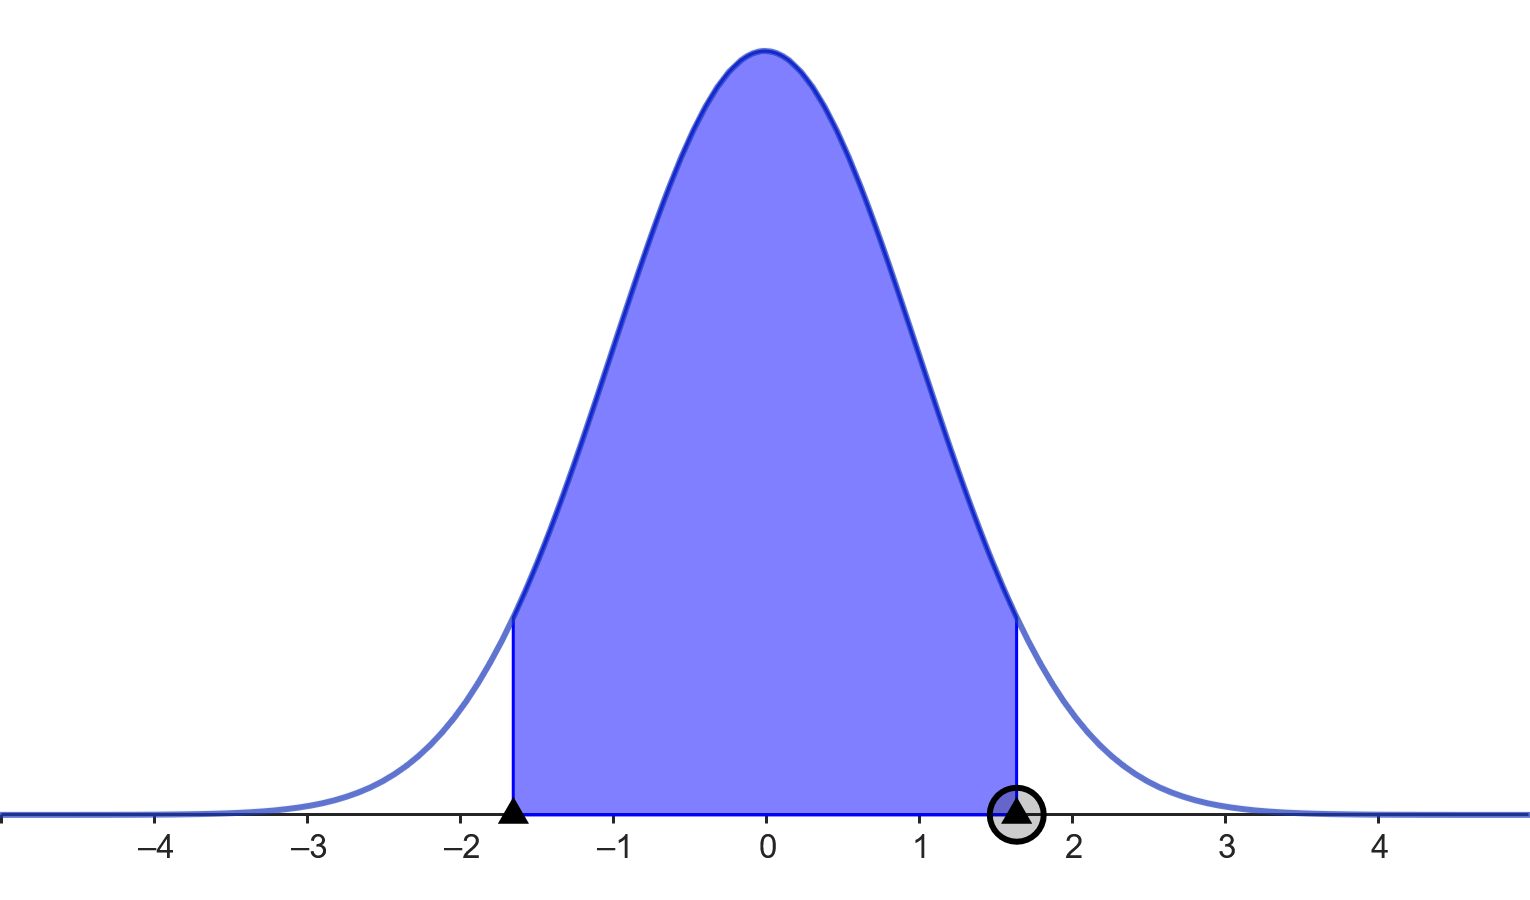
\includegraphics[width=8cm]{Bilder/geogebra-export.png}
  \centering
\end{figure}


\section{Konzept Analysetool}
Das Analysetool wird mit den Logs des Fio-Tools analysieren.
Das Fio-Too durchläuft 5 - 10 mal die gleichen Tests, wo dann der stationäre Zustand, des Analysetools,
bestimmt werden soll. Das Tool wird in der Lage mit den drei Tests die eingeführt zu arbeiten.
Da die Anzahl nicht festgelegt werden kann, da die dieser Zustand an einem unbestimmten Zeitpunkt und Iteration erreicht wird,
werden verschiedene Anläufe getestet mit einer verschieden Anzahl and Fio-Tool Testanzahl.

